\appendix
\setcounter{MaxMatrixCols}{20}
\chapter{Программа расчета параметров математическо модели ленточного конвейера} \label{Appendix0}
\begin{verbatim}
format long
% переменные
    % длина конвейера / 2
    l   = 500;
    % погонный вес движущихся частей на грузовой ветви, Н/м
    Gg  = 104.5;
    % погонный вес движущихся частей на порожней ветви, Н/м
    Gp  = 25;
    % вес натяжного устройства, Н
    G   = 80000;
    % масса участка грузовой ветви, кг
    mg  = 870.8;
    % масса участка порожней ветви, кг
    mp  = 208.3;
    % масса привода, кг
    mpr = 2850;
    M   = 1;
    P   = 110000;
    % радиус барабана, м
       R   = 0.4;
    % коэффициент сопротивления движению
    w   = 0.03;
    % коэффициент сопротивления движению натяжных грузов
    f   = 0.3;
    % вязкость енты, Н/м
    eta = 1100;
    % жесткость ленты, Н/м
    C   = 1000;
    % жесткость канатов натяжного устройства, Н/м
    Ck  = 5*10^5;
    % ускорение свободного падения, м/с^2
    g   = 9.8;
% ____________

% матрица при вторых производных X, mtM 5x5
mtM  = [2*mg+2*mp+mpr mg 0 mp; mg 4*mg mg 0; 0 mg 2*mg+2*mp mp;
        mp 0 mp 4*mp];

% матрица при перых производных X, определяющая вязкости, mtN 5x5
mtN  = [2*eta -eta 0 -eta; -eta 2*eta -eta 0; 0 -eta 2*eta -eta;
        -eta 0 -eta 2*eta];

% матрица при координатах X, определяющая жесткости, mtС 5x5
mtC  = [2*C -C 0 -C; -C 2*C -C 0; 0 -C 2*C+0.25*Ck -C-0.25*Ck;
        -C 0 -C-0.25*Ck 2*C+0.25*Ck];

% матрица при SGN(X), определяющая силы сопротивления, mtS 5x5
mtS  = [0.5*Gg*l*w + 0.5*Gp*l*w 0 0 0; 0 Gg*l*w 0 0;
        0 0 0.5*Gg*l*w + 0.5*Gp*l*w 0; 0 0 0 Gp*l*w];

% матрица, связанная с приводом, mtP1 5x1
mtP1 = [1/R; 0; 0; 0;];

% матрица, связанная с тормознвм моментом приводного барабана, mtP2 5x1
mtP2 = [-1/R; 0; 0; 0];

% матрица, связанная с тормознвм моментом хвостового барабана, mtP3 5x1
mtP3 = [0; 0; -1/R; 0];

% матрица mtG 5x1
mtG  = [0; 0; -0.5*Ck; 0.5*Ck];

% Z   - нулевая матрица 5x5
% E   - единичная матрица 5x5
% ZZ  - нулевая матрица 5x1
% ZZZ - нулевая матрица 5x10
Z    = zeros(4);
E    = eye(4);
ZZ   = zeros(4,1);
ZZZ  = zeros(4,8);

% матрица состояния системы, А 8x8
A    = -[Z -E; (mtM^(-1))*mtC (mtM^(-1))*mtN];

% матрица управления системы, В 8x12
% конкатенация: cat(dim, A, B)
% dim == 1 - вертикальная конкатенация
% dim == 2 - горизонтальная конкатенация
B    = cat(2,
           cat(1, ZZ, (mtM^-1)*mtP1),
           cat(1, 
               ZZZ,
               cat(2, Z, -(mtM^-1)*mtS)
              ),
           cat(1, 
               ZZ, 
               -(mtM^-1)*mtG
              ),
           cat(1,
               ZZ,
               (mtM^-1)*mtP2
              ),
           cat(1, 
               ZZ,
               (mtM^-1)*mtP3
              )
          );

% матрица выхода модели, С 8x8
C    = eye(8);
D    = zeros(8,12);
\end{verbatim}

\chapter{Числовые значения матриц} \label{Appendix1}
\section{Числовые значения матриц системы уравнений, описывающей исходную математическую модель ленточного конвейера}\label{Appendix11}

$ 
M = 
\begin{bmatrix}
	4008,2 & 870,9  & 0      & 208,3 & 0    \\
	807,8  & 3483,2 & 870,8  & 0     & 0    \\
	0      & 870,8  & 2158,2 & 208,3 & 0    \\
	208,3  & 0      & 208,3  & 833,2 & 0    \\
	0      & 0      & 0      & 0     & 3000
\end{bmatrix},
$
\bigskip

$
N = 
\begin{bmatrix}
	2200  & -1100 & 0     & -1100 & 0       \\
	-1100 & 2200  & -1100 & 0     & 0       \\
	0     & -1100 & 2200  & -1100 & 0       \\
	-1100 & 0     & -1100 & 2200  & 0       \\
	0     & 0     & 0     & 0     & 0
\end{bmatrix},
$
\bigskip

$ 
C = 
\begin{bmatrix}
	2000  & -1000 & 0       & -1000   & 0       \\
	-1000 & 2000  & -1000   & 0       & 0       \\
	0     & -1000 & 127000  & -126000 & -250000 \\
	-1000 & 0     & -126000 & 127000  & 250000  \\
	0     & 0     & -250000 &  250000 & 500000
\end{bmatrix},
$
\bigskip

$
 P = 
\begin{bmatrix}
	2                                \\
	0                                \\
	0                                \\
	0                                \\
	0
\end{bmatrix}, G = 
\begin{bmatrix}
	0                                \\
	0                                \\
	0                                \\
	0                                \\
	30000
\end{bmatrix},
$

\bigskip

$ S =
\begin{bmatrix}
 971,2 & 0      & 0     & 0   & 0        \\
 0     & 1567,5 & 0     & 0   & 0        \\
 0     & 0      & 971,2 & 0   & 0        \\
 0     & 0      & 0     & 375 & 0        \\
 0     & 0      & 0     & 0   & 0 2235 
\end{bmatrix}.
$

\section{Числовые значения матриц исходной внутренней модели ленточного конвейера}\label{Appendix12}

$
\tilde{A}_{10\times10} = 
\begin{bmatrix}
0     & 0     & 0      & 0       & 0       & 1     & 0     & 0     & 0     & 0 \\
0     & 0     & 0      & 0       & 0       & 0     & 1     & 0     & 0     & 0 \\
0     & 0     & 0      & 0       & 0       & 0     & 0     & 1     & 0     & 0 \\
0     & 0     & 0      & 0       & 0       & 0     & 0     & 0     & 1     & 0 \\
0     & 0     & 0      & 0       & 0       & 0     & 0     & 0     & 0     & 1 \\
-0,70 & 0,46  & -14,71 & 14,94   & 28,96   & -0,76 & 0,51  & -0,25 & 0,51  & 0 \\
0,55  & -0,90 & 25,50  & -25,15  & -49,64  & 0,60  & -0,99 & 0,75  & -0,36 & 0 \\
-0,36 & 0,86  & -86,17 & 85,67   & 169,62  & -0,40 & 0,95  & -1,49 & 0,95  & 0 \\
1,46  & -0,33 & 176,44 & -177,58 & -349,70 & 1,61  & -0,36 & 1,76  & -3,00 & 0 \\
0     & 0     & 35,00  & -35,00  & -70,00  & 0     & 0     & 0     & 0     & 0
\end{bmatrix},
$
\bigskip

$
\tilde{B_1}_{10\times1} = 
\begin{bmatrix}
0       \\
0       \\
0       \\
0       \\
0       \\
675,70  \\
-193,06 \\
96,53   \\
-193,06 \\
0
\end{bmatrix},
$
\bigskip

$
\tilde{B_2}_{10\times10} = 
\begin{bmatrix}
0 & 0 & 0 & 0 & 0 & 0     & 0     & 0     & 0     & 0 \\
0 & 0 & 0 & 0 & 0 & 0     & 0     & 0     & 0     & 0 \\
0 & 0 & 0 & 0 & 0 & 0     & 0     & 0     & 0     & 0 \\
0 & 0 & 0 & 0 & 0 & 0     & 0     & 0     & 0     & 0 \\
0 & 0 & 0 & 0 & 0 & 0     & 0     & 0     & 0     & 0 \\
0 & 0 & 0 & 0 & 0 & -0,26 & 0,12  & -0,04 & 0,03  & 0 \\
0 & 0 & 0 & 0 & 0 & 0,08  & -0,54 & 0,14  & -0,02 & 0 \\
0 & 0 & 0 & 0 & 0 & -0,04 & 0,22  & -0,52 & 0,05  & 0 \\
0 & 0 & 0 & 0 & 0 & 0,08  & -0,09 & 0,14  & -0,47 & 0 \\
0 & 0 & 0 & 0 & 0 & 0     & 0     & 0     & 0     & -2,94
\end{bmatrix},
$
\bigskip

$
\tilde{B_3}_{10\times1} = 
\begin{bmatrix}
0       \\
0       \\
0       \\
0       \\
0       \\
0       \\
0       \\
0       \\
0       \\
-9,8    
\end{bmatrix}.
$

\section{Числовые значения матриц системы уравнений, описывающей движение ленты конвейера отдельно от натяжного устройтсва}\label{Appendix13}

$
M = 
\begin{bmatrix}
	4008,2 & 870,8  & 0      & 208,3 \\
	870,8  & 3483,2 & 870,8  & 0     \\
	0      & 870,8  & 2158,2 & 208,3 \\
	208,3  & 0      & 208,3  & 833,2 
\end{bmatrix}, N = 
\begin{bmatrix}
	2200  & -1100 & 0     & -1100    \\
	-1100 & 2200  & -1100 & 0        \\
	0     & -1100 & 2200  & -1100    \\
	-1100 & 0     & -1100 & 2200                                   
\end{bmatrix},
$
\bigskip

$
P = 
\begin{bmatrix}
	2,5                               \\
	0                                 \\
	0                                 \\
	0                      
\end{bmatrix}, B_1 = 
\begin{bmatrix}
	0                                 \\
	0                                 \\
	-250000                           \\
	250000
\end{bmatrix}, C = 
\begin{bmatrix}
	2000  & -1000 & 0       & -1000   \\
	-1000 & 2000  & -1000   & 0       \\
	0     & -1000 & 127000  & -126000 \\
	-1000 & 0     & -126000 & 127000   
\end{bmatrix},
$
\bigskip

$
S = 
\begin{bmatrix}
	971,25 & 0      & 0      & 0     \\
	0      & 1567,5 & 0      & 0     \\
	0      & 0      & 971,25 & 0     \\
	0      & 0      & 0      & 375  
\end{bmatrix}.
$

\section{Числовые значения матриц внутренней модели движения ленты конвейера отдельно от натяжного устройтсва}\label{Appendix14}

$
A_{[8 \times 8]} = 
\begin{bmatrix}
 0     & 0     & 0      & 0       & 1     & 0     & 0     & 0     \\
 0     & 0     & 0      & 0       & 0     & 1     & 0     & 0     \\
 0     & 0     & 0      & 0       & 0     & 0     & 1     & 0     \\ 
 0     & 0     & 0      & 0       & 0     & 0     & 0     & 1     \\
 -0,70 & 0,46  & -14,71 & 14,94   & -0,76 & 0,51  & -0,25 & 0,51  \\
 0,55  & -0,91 & 25,51  & -25,15  & 0,61  & -0,99 & 0,75  & -0,36 \\
 -0,36 & 0,86  & -86,17 & 85,67   & -0,40 & 0,95  & -1,49 & 0,95  \\
 1,47  & -0,33 & 176,44 & -177,58 & 1,61  & -0,36 & 1,76  & -3,00
\end{bmatrix}.
$
\bigskip

$
{B_\text{пр}}_{[8 \times 1]} = 
\begin{bmatrix}
0        \\
0        \\
0        \\
0        \\
0,00068  \\
-0,00019 \\
0,000097 \\
-0,00019
\end{bmatrix}, 
$
\bigskip

$
{B_s}_{[8 \times 8]} = 
\begin{bmatrix}
 0 & 0 & 0 & 0 & 0     & 0     & 0     & 0     \\
 0 & 0 & 0 & 0 & 0     & 0     & 0     & 0     \\
 0 & 0 & 0 & 0 & 0     & 0     & 0     & 0     \\ 
 0 & 0 & 0 & 0 & 0     & 0     & 0     & 0     \\
 0 & 0 & 0 & 0 & -0,26 & 0,12  & -0,04 & 0,03  \\
 0 & 0 & 0 & 0 & 0,08  & -0,54 & 0,14  & -0,02 \\
 0 & 0 & 0 & 0 & -0,04 & 0,22  & -0,52 & 0,05  \\ 
 0 & 0 & 0 & 0 & 0,08  & -0,09 & 0,14  & -0,47 \\
\end{bmatrix}, 
$
\bigskip

$
{B_1}_{[8 \times 1]} = 
\begin{bmatrix}
 0       \\
 0       \\
 0       \\
 0       \\
 28,96   \\
 -49,64  \\
 169,62  \\
 -349,69 \\
\end{bmatrix}.
$

\section{Числовые значения матрицы управления модифицированной модели движения ленты конвейера}\label{Appendix15}

$
B_{[8 \times 12]} = 
\begin{bmatrix}
 0       & 0 & 0 & 0 & 0 & 0     & 0    & 0     & 0     & 0       & 0        & 0      \\
 0       & 0 & 0 & 0 & 0 & 0     & 0    & 0     & 0     & 0       & 0        & 0      \\
 0       & 0 & 0 & 0 & 0 & 0     & 0    & 0     & 0     & 0       & 0        & 0      \\
 0       & 0 & 0 & 0 & 0 & 0     & 0    & 0     & 0     & 0       & 0        & 0      \\
 0,00068 & 0 & 0 & 0 & 0 & -0,26 & 0,12 & -0,04 & 0,029 & 28,96   & -0,00068 & -9,65  \\
 -0,0002 & 0 & 0 & 0 & 0 & 0,08  & -0,4 & 0,14  & -0,02 & -49,64  & 0,0002   & 0,0004 \\
 0,00009 & 0 & 0 & 0 & 0 & -0,04 & 0,22 & -0,52 & 0,05  & 169,62  & -0,00009 & -0,001 \\
 -0,0002 & 0 & 0 & 0 & 0 & 0,08  & -0,9 & 0,14  & -0,47 & -349,69 & 0,0002   & 0,0004 \\
\end{bmatrix}.
$

\chapter{Исходный код программы вычисления зависимостей натяжений в ленте от ее деформаций} \label{AppendixLSM} 
\begin{verbatim}
\% least-squares method for S1 and S4
delta1 = [4.25  5.5   6.76  8.01  8.64  9.26  9.75  10.6  11.12
          11.74 12.36]
S1     = [41200 46200 51200 56200 58700 61200 63700 66200 68700 
          71200 73700]

delta4 = [1.34  2.59  3.85  5.1   5.72  6.35  6.99  7.59  8.21 
          8.83  9.45 ]
S4     = [2500  7500  12500 17500 20000 22500 25000 27500 30000 
          32500 35000]

p1     = polyfit(delta1, S1, 1)
p4     = polyfit(delta4, S4, 1)

xx1    = linspace(delta1(1), delta1(end), 100)
yy1    = polyval(p1, xx1)

xx4    = linspace(delta4(1), delta4(end), 100)
yy4    = polyval(p4, xx4)

figure;
subplot(1,2,1)
plot(delta1, S1, 'o', xx1, yy1)

subplot(1,2,2)
plot(delta4, S4, 'o', xx4, yy4)
\end{verbatim}

\chapter{Исходные коды программ реализации алгоритмов управления} \label{AppendixB}                      

\section{Исходный код расчета параметров управляющих алгоритмов} \label{AppendixB1}
\fontsize{11pt}{12pt}\selectfont

\begin{verbatim}
(*
 *
 * IEC 61131-3 Structured Text (ST) code
 * Model creator                   : Roman Bukharov
 * Simulink PLC Coder version      : 1.4 (R2012b) 20-Jul-2012
 * Target IDE selection            : Siemens SIMATIC Step 7 5.4
 *
 *)
FUNCTION_BLOCK FB44
    VAR_INPUT
    END_VAR
    
    VAR_OUTPUT
        E0ma_nominal: REAL;
        E0ma_brake  : REAL;
        MT_tail     : REAL;
        MT_drive    : REAL;
    END_VAR
    
    VAR
        Wt          : REAL;
    END_VAR
    
    CONST
        // Belt grasp angle 
        alpha       := 3.14;
        // Traction coefficient 
        mu          := 0.25;
        // Safety factor 
        k_t         := 1.1;
        // Belt weight 
        ql          := 100;
        // Roller supports weight 
        qr          := 150;
        // Tension of empty branch 
        Sup         := 32456;
        // Tension of load branch 
        Sug         := 71152;
        // Brake disk radius 
        R           := 0.4;
        // Pull device weight 
        Gnu         := 80000;
        // Conveyor length 
        L           := 1000;
        // Coefficient of resistance movement 
        w           := 0.03;
    END_CONST
    
    // Pull factor (normal mode) nominal value 
    E0ma_nominal := k_t * EXP(mu * alpha);
    // Pull factor (brake mode) nominal value 
    E0ma_brake := 1 / E0ma_nominal;
    // Wt calculation
    Wt := (Sup - E0ma_brake * Sug) / (E0ma_brake + 1.0);
    // Tail brake moment calculation 
    MT_tail := 0.5 * R * (0.5 * Gnu - (ql + qr) * L * w - Sup + Wt);
    // Drive brake moment calculation
    MT_drive := 4 * MT_tail / R;
END_FUNCTION_BLOCK

\end{verbatim}

\section{Исходный код функционального блока вычисления текущего значения тягового фактора} \label{AppendixB2}
\fontsize{11pt}{12pt}\selectfont

\begin{verbatim}
(*
 *
 * IEC 61131-3 Structured Text (ST) code
 * Model creator                   : Roman Bukharov
 * Simulink PLC Coder version      : 1.4 (R2012b) 20-Jul-2012
 * Target IDE selection            : Siemens SIMATIC Step 7 5.4
 *
 *)
FUNCTION_BLOCK FB11
    VAR_INPUT
        x5           : REAL;
        x6           : REAL;
        x7           : REAL;
        x8           : REAL;
    END_VAR
    
    VAR_OUTPUT
        Ema_1        : REAL;
        Ema_2        : REAL;
        S1_2         : REAL;
        S4_2         : REAL;
    END_VAR
    
    VAR
        S4           : REAL;
        S1           : REAL;
        rtb_Product1 : REAL;
    END_VAR
    
    CONST
        S1_a         := 4006.9;
        S1_b         := 24130.5;
        S4_a         := 4005.6;
        S4_b         := -2904.7;
    END_CONST
    
    // S1 tension
    S1 := ((x5 - x6) * S1_a) + S1_b;
    // S4 tension
    S4 := (((x8 - x5) * S4_a) + S4_b);
    // E_ma
    rtb_Product1 := S1 / S4;
    // Saturation (E_ma (nominal mode))
    IF rtb_Product1 >= 20.0 THEN 
        // max 
        Ema_1 := 20.0;
    ELSIF rtb_Product1 > -20.0 THEN 
        // default 
        Ema_1 := rtb_Product1;
    ELSE 
        // min 
        Ema_1 := -20.0;
    END_IF;
    // S1 output
    S1_2 := S1;
    // S4 output
    S4_2 := S4;
    // E_ma (brake mode)
    Ema_2 := 1 / Ema_1;
END_FUNCTION_BLOCK
\end{verbatim}

\section{Исходный код функционального блока реализации алгоритма предварительного торможения конвейера} \label{AppendixB3}
\fontsize{11pt}{12pt}\selectfont

\begin{verbatim}
(*
 *
 * IEC 61131-3 Structured Text (ST) code
 * Model creator                   : Roman Bukharov
 * Simulink PLC Coder version      : 1.4 (R2012b) 20-Jul-2012
 * Target IDE selection            : Siemens SIMATIC Step 7 5.4
 *
 *)
FUNCTION_BLOCK FB22
    VAR_INPUT
        enable            : BOOL;
        v1                : REAL;
        v3                : REAL;
        Ema               : REAL;
        Ema_max           : REAL;
        _brakemomenttail  : REAL;
        _brakemomentdrive : REAL;
    END_VAR
    
    VAR_OUTPUT
        brakemomenttail   : REAL;
        drivestop         : REAL;
        brakemomentdrive  : REAL;
    END_VAR
    
    VAR
    END_VAR
    
    VAR_TEMP
        y: REAL;
    END_VAR
    
    CONST 
    END_CONST    
    
    IF enable = TRUE THEN
        // Sign (v3)
        IF v3 < 0.0 THEN 
            y := -1.0;
        ELSIF v3 > 0.0 THEN 
            y := 1.0;
        ELSE 
            y := v3;
        END_IF;
        // brake moment (tail) calculation
        brakemomenttail := _brakemomenttail * y;        
        // drive stopping
        IF Ema > Ema_max THEN
            drivestop := 0;
        ELSE 
            drivestop := 1;
        END_IF;  
        // brake moment (drive)
        IF v1 > 0.01 THEN 
            // null
            brakemomentdrive := 0.0;
        ELSE 
            // Sign (v1)
            IF v1 < 0.0 THEN 
                y := -1.0;
            ELSIF v1 > 0.0 THEN 
                y := 1.0;
            ELSE 
                y := v1;
            END_IF;
            // brake moment (drive) calculation
            brakemomentdrive := _brakemomentdrive * y;
        END_IF;       
    ELSE
        drivestop        := 0;
        brakemomentdrive := 0;
        brakemomenttail  := 0;
    END_IF;
END_FUNCTION_BLOCK
\end{verbatim}

\section{Исходный код функционального блока реализации регулятора натяжения ленты конвейера} \label{AppendixB4}

\begin{verbatim}
(*
 *
 * IEC 61131-3 Structured Text (ST) code
 * Model creator                   : Roman Bukharov
 * Simulink PLC Coder version      : 1.4 (R2012b) 20-Jul-2012
 * Target IDE selection            : Siemens SIMATIC Step 7 5.4
 *
 *)
FUNCTION_BLOCK fb66
    VAR_INPUT
        Ema      : REAL;
        E0ma     : REAL;
    END_VAR
    
    VAR_OUTPUT
        Movement : REAL;
    END_VAR
    
    VAR
        Weight   : REAL;
    END_VAR
    
    CONST
        Weight_a   := 22230.0;
        Weight_b   := 149540.0;
        Weight_c   := 3013810.0;

        Movement_a := 0.0002;
        Movement_b := 0.4257;
    END_CONST
    
    // Weight calculation
    Weight := (((( -(Ema - E0ma)) + E0ma) ** 2.0 * Weight_a) - 
              ((( -(Ema - E0ma)) + E0ma) * Weight_b)) + Weight_c;
    // Saturate
    IF Weight >= 100000.0 THEN 
        Weight := 100000.0; 
    ELSIF  NOT (weight > -100000.0) THEN 
        Weight := -100000.0;
    END_IF;
    // Movement calculation
    Movement   := (Movement_a * Weight) + Movement_b;
END_FUNCTION_BLOCK
\end{verbatim}

\section{Исходный код функционального блока реализации интегратора} \label{AppendixB5}
\begin{verbatim}
FUNCTION_BLOCK FB70
    // Integral calculation 
    VAR_INPUT
        IN          : REAL;
        RESET       : BOOL;
        ENABLE      : BOOL;
    END_VAR
    
    VAR_OUTPUT
        OUT         : REAL;
        RESET_ACTIV : BOOL;
    END_VAR    
    
    VAR
        OUT_LOW     : REAL;
        LAST_IN     : REAL;
        LAST_OUT    : REAL;
        LAST_TIME   : REAL;
        ACTUAL_TIME : REAL;
        X : REAL;
        n : INT;
    END_VAR
    
    // Reset of values
    RESET_ACTIV := RESET;
    IF RESET = TRUE THEN
        OUT         := 0.0;
        OUT_LOW     := 0.0;
        LAST_OUT    := 0.0;
        LAST_TIME   := ACTUAL_TIME;
        ACTUAL_TIME := TIME_TO_DINT(TIME_TCK()) / 1000.0;
        X           := 0.0;
        n           := 0;
    ELSIF ENABLE = FALSE THEN
        n           := 0;   
    ELSE
        //First Integral Cyclus
        IF n = 0 THEN
                ACTUAL_TIME := TIME_TO_DINT(TIME_TCK()) / 1000.0;
                LAST_TIME   := ACTUAL_TIME;
                LAST_IN     := IN;
                n           := 1;
        ELSE  
            // Input 
            ACTUAL_TIME     := TIME_TO_DINT(TIME_TCK()) / 1000.0;
            
            // Overflow Correction
            IF ACTUAL_TIME < LAST_TIME THEN
                X           := (ACTUAL_TIME - LAST_TIME + 2147483.647) *
                               (IN + LAST_IN) / 2; 
            ELSE
                X           := (ACTUAL_TIME - LAST_TIME) * 
                               (IN + LAST_IN) / 2;
            END_IF;
        
            LAST_TIME       := ACTUAL_TIME;
            LAST_IN         := IN;
    
            // Integral Calculation
            LAST_OUT        := OUT;
            OUT             := LAST_OUT + X; 
            OUT_LOW         :=  (OUT - LAST_OUT) - X + OUT_LOW;
    
            IF OUT_LOW <> 0 THEN
                IF ABS(OUT/OUT_LOW) < 10000000 THEN
                    LAST_OUT := OUT;
                    OUT      := OUT  - OUT_LOW;
                    OUT_LOW  := (OUT - LAST_OUT) + OUT_LOW;
                END_IF;
            END_IF;
        END_IF;
    END_IF;
END_FUNCTION_BLOCK
\end{verbatim}

\section{Исходный код функционального блока реализации оптимального регулятора скорости движения ленты конвейера} \label{AppendixB6}
\begin{verbatim}
(*
 *
 * IEC 61131-3 Structured Text (ST) code
 * Model creator                   : Roman Bukharov
 * Simulink PLC Coder version      : 1.4 (R2012b) 20-Jul-2012
 * Target IDE selection            : Siemens SIMATIC Step 7 5.4
 *
 *)
FUNCTION_BLOCK FB77
    VAR_INPUT
        // belt speed value
        V0       : REAL;
        // integral of belt speed value
        V0_int   : REAL;
        // start signal
        start    : BOOL;
        //speeds
        v1       : REAL;
        v2       : REAL;
        v3       : REAL;
        v4       : REAL;
        v5       : REAL;
        // coordinates
        x1       : REAL;
        x2       : REAL;
        x3       : REAL;
        x4       : REAL;
        x5       : REAL;
    END_VAR

    VAR_OUTPUT
        // control signal
        w        : REAL;
        // drive start
        _start   : BOOL;
    END_VAR

    VAR
        // K matrix
        Feedback : ARRAY[1..10, 1..3] OF REAL :=
                 0    ,0    ,0   ,0   ,0   ,0    ,0    ,0    ,0    ,0,
                 0    ,0    ,0   ,0   ,0   ,0    ,0    ,0    ,0    ,0,
                 108.5,116.6,69.8,23.5,4.03,668.5,771.6,485.5,190.7,96.1;
        // -eye(10)*inv(A-B*UPR)*U
        V        : ARRAY[1..1, 1..10] OF REAL := 
                 25.388,
                 32.487,
                 34.362,
                 28.000,
                 3.201,
                 -1,
                 -1,
                 -1,
                 -1,
                 -1;
        // U matrix
        U        : ARRAY[1..1, 1..10] OF REAL := 
                 -1,
                 -1,
                 -1,
                 -1,
                 -1,
                 -1,
                 -1,
                 -1,
                 -1,
                 -1;   
        // State coordinates
        Coords   : ARRAY[1..1, 1..10] OF REAL;
        // Control signals matrix
        Control  : ARRAY[1..1, 1..3]  OF REAL;
        // temporary variables
        Sum1, 
        Sum2, 
        Sum3     : ARRAY[1..1, 1..10] OF REAL;
        Sum4     : ARRAY[1..3, 1..10] OF REAL;
    END_VAR

    VAR_TEMP
        // iterators
        row      : INT;
        col      : INT;
        inner    : INT;
    END_VAR

    CONST
    END_CONST
    
    // enable drive
    _start := start;
    IF start THEN
        // state coordinates
        Coords[1,1]  := x1;
        Coords[1,2]  := x2;
        Coords[1,3]  := x3;
        Coords[1,4]  := x4;
        Coords[1,5]  := x5;
        Coords[1,6]  := v1;
        Coords[1,7]  := v2;
        Coords[1,8]  := v3;
        Coords[1,9]  := v4;
        Coords[1,10] := v5;
        FOR col := 1 TO 10 BY 1 DO
           //input and -eye(10)*inv(A-B*UPR)*U product
           Sum1[1, col] := 0.13*V0*V[1, col];
           //integral input and U matrix product
           Sum2[1, col] := 0.13*V0_int*U[1, col];            
        END_FOR;
        // 
        FOR col := 1 TO 10 BY 1 DO
           Sum3[1, col] := Coords[1, col] - Sum1[1, col];
        END_FOR;
        //
        FOR col := 1 TO 10 BY 1 DO
           Sum4[1, col] := Sum3[1, col] + Sum2[1, col];
        END_FOR;
        // Control signals matrix calculation
        FOR row := 1 TO 10 BY 1 DO
            FOR col := 1 TO 3 BY 1 DO
                FOR inner := 1 TO 3 BY 1 DO
                    Control[row,col] := Feedback[row,inner] *
                                        Sum4[inner,col];
                END_FOR;
            END_FOR;
        END_FOR;
        // Output
        w := Control[1,3];    
    END_IF;
END_FUNCTION_BLOCK
\end{verbatim}

\section{Список переменных программы управляющего контроллера} \label{AppendixB7}
%\fontsize{14pt}{15pt}\selectfont

\begin{table}[h!]
\caption{Список переменных программы управляющего контроллера}
\label{5.tabl:variables}
 
\begin{center}
\begin{tabular}{|p{0.25\linewidth}|p{0.1\linewidth}|p{0.1\linewidth}|p{0.35\linewidth}|}
\hline
Имя переменной           & Адрес  & Тип    &  Комментарий                                                 \\
\hline
Pull factor              & FB 11  & FB 11  & Функциональный блок вычисления текущего значения тягового фактора \\
\hline 
Brake algorithm          & FB 22  & FB 22  & Функциональный блок алгоритма торможения конвейера           \\
\hline 
Initialization           & FB 44  & FB 44  & Функциональный блок вычисления начальных параметров          \\
\hline 
Derivative               & FB 55  & FB 55  & Функциональный блок реализации дифференцирования             \\
\hline 
Pull device control      & FB 66  & FB 66  & Функциональный блок алгоритма стабилизации тягового фактора  \\
\hline 
Integrator               & FB 70  & FB 70  & Функциональный блок реализации интегрирования                \\
\hline  
Speed control            & FB 77  & FB 77  & Функциональный блок оптимального регулятора скорости         \\
\hline   
input start              & I  1.0 & BOOL   & Сигнал пуска конвейера (вход)                                \\
\hline    
x1                       & MD 100 & REAL   & Перемещение в первой характерной точке ленты                 \\
\hline  
x2                       & MD 104 & REAL   & Перемещение во второй характерной точке ленты                \\
\hline  
x3                       & MD 108 & REAL   & Перемещение в третьей характерной точке ленты                \\
\hline  
x4                       & MD 112 & REAL   & Перемещение в четвертой характерной точке ленты              \\
\hline  
x5                       & MD 116 & REAL   & Перемещение натяжного устройства                             \\
\hline  
 

\end{tabular}
\end{center}
\end{table}


\begin{table}[h!]
%\caption{Продолжение}

\begin{center}
\begin{tabular}{|p{0.25\linewidth}|p{0.1\linewidth}|p{0.1\linewidth}|p{0.35\linewidth}|} 
\hline
brake                    & ID 128 & REAL   & Сигнал включения процесса останова                           \\
\hline  
omega                    & ID 132 & REAL   & Сигнал управления оптимального регулятора скорости           \\
\hline  
V0                       & ID 136 & REAL   & Задание скорости движения ленты                              \\
\hline 
V1                       & ID 100 & REAL   & Скорость первой характерной точки ленты                      \\
\hline  
V2                       & ID 104 & REAL   & Скорость второй характерной точки ленты                      \\
\hline  
V3                       & ID 108 & REAL   & Скорость третьей характерной точки ленты                     \\
\hline  
V4                       & ID 112 & REAL   & Скорость четвертой характерной точки ленты                   \\
\hline  
V5                       & ID 116 & REAL   & Скорость натяжного устройства                                \\
\hline  
V0 int                   & MD 120 & REAL   & Интеграл задания скорости движения ленты                     \\
\hline  
Cycle execution          & OB 1   & OB 1   & Блок циклического выполнения основной программы              \\
\hline  
CYC INT5                 & OB 35  & OB 35  & Блок выполнения программы по прерыванию времени              \\
\hline  
COMPLETE RESTART         & OB 100 & OB 100 & Блок выполнения программы при запуске контроллера            \\
\hline  
output start             & Q  1.0 & BOOL   & Сигнал пуска конвейера (выход)                               \\
\hline  
Ema brake                & QD 100 & REAL   & Текущее значение тягового фактора для режима торможения      \\
\hline  
Ema nominal              & QD 104 & REAL   & Текущее значение тягового фактора для номинального режима    \\
\hline  
S1 2                     & QD 108 & REAL   & Текущее значение натяжения ленты в точке набегания           \\
\hline   
S4 2                     & QD 112 & REAL   & Текущее значение натяжения ленты в точке сбегания            \\
\hline  
brake tail               & QD 116 & REAL   & Значение тормозного момента для хвостового барабана (выход)  \\
\hline  
brake drive              & QD 120 & REAL   & Значение тормозного момента для приводного барабана  (выход) \\
\hline   
stop                     & QD 124 & REAL   & Сигнал останова привода                                      \\
\hline  
\_Ema brake max          & QD 128 & REAL   & Задание значения тягового фактора для режима торможения      \\
\hline  
\_Ema nominal min        & QD 132 & REAL   & Задание значение тягового фактора для номинального режима    \\
\hline  
\_brake moment drive nom & QD 136 & REAL   & Значение тормозного момента для приводного барабана (задание)\\
\hline  
\_brake moment tail nom  & QD 140 & REAL   & Значение тормозного момента для хвостового барабана (задание)\\
\hline  
Pull device movement     & QD 152 & REAL   & Перемещение натяжного устройства (выход)                     \\
\hline  
drive control            & QD 156 & REAL   & Управление приводом                                          \\
\hline   
TIME\_TCK                & SFC 64 & SFC 64 & Системное время                                              \\ 
\hline 
\end{tabular}
\end{center}
\end{table}     
\clearpage

\section{Исходный код основной управляющей программы} \label{AppendixB8}
%\fontsize{14pt}{15pt}\selectfont

Основной блок OB1 (циклическое исполнение):

\begin{figure} [h!] 
  \center
  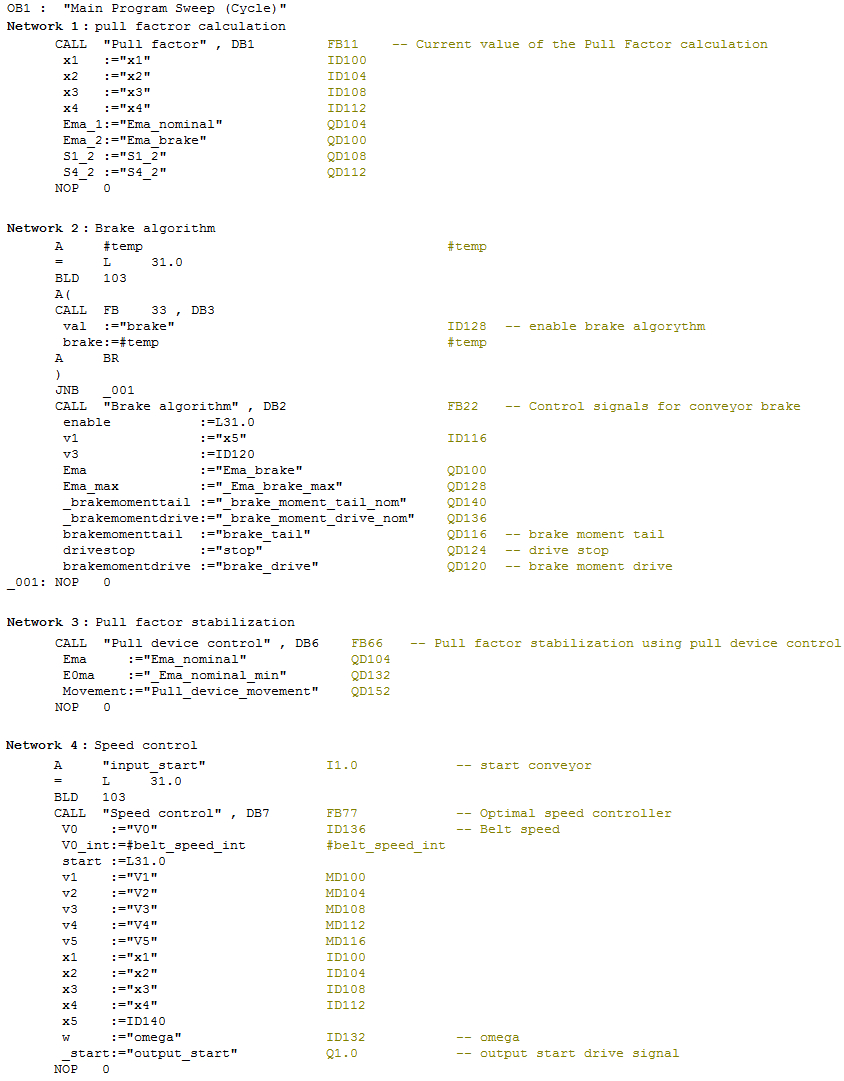
\includegraphics [scale=0.8] {main_program.png}
  \label{img.5.main_program}  
\end{figure}

Блок OB100 (исполнение при запуске контроллера):

\begin{figure} [h!] 
  
  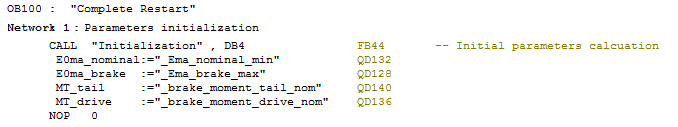
\includegraphics [scale=0.8] {init_program.png}
  \label{img.5.init_program}  
\end{figure}

Блок OB135 (исполнение по циклическому прерыванию каждые 100 мс):

\begin{figure} [h!] 
  
  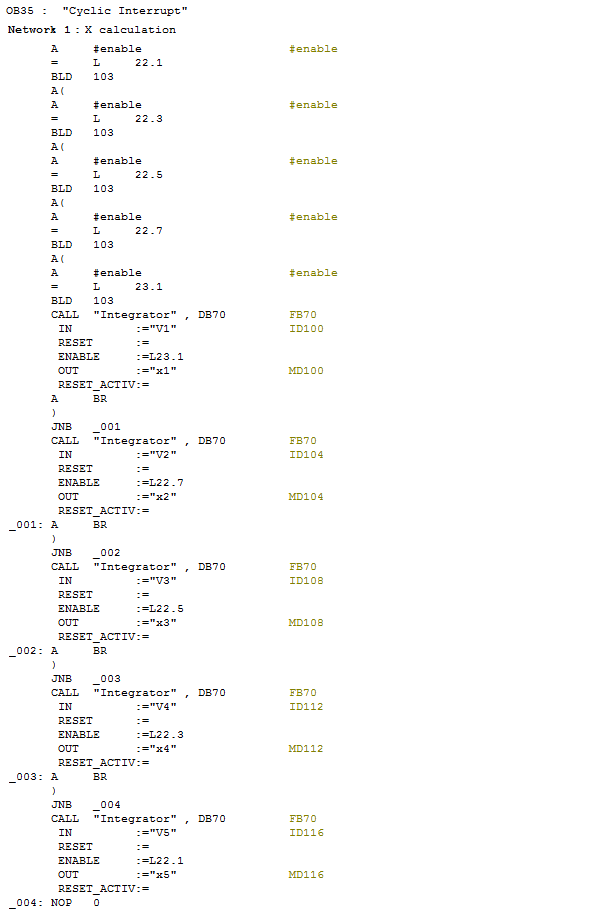
\includegraphics [scale=0.82] {interrupt_program.png}
  \label{img.5.interrupt_program}  
\end{figure}
\clearpage
\begin{figure} [h!] 
  
  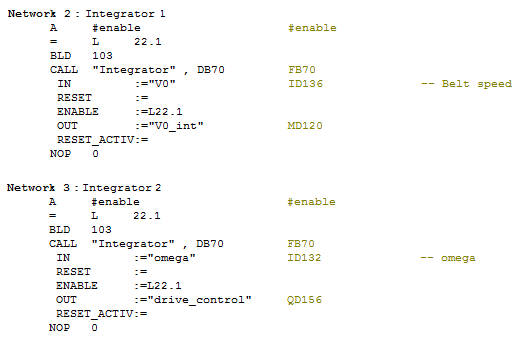
\includegraphics [scale=0.8] {interrupt_program1.png}
  \label{img.5.interrupt_program1}  
\end{figure}
\textcolor{white}{\_\_}